% \documentclass[11pt]{article}
\documentclass[10pt,twocolumn]{article}  %10pt is big enough with lucida
\usepackage{graphicx}
\usepackage{placeins}
\usepackage{url}
\widowpenalty10000

% LLS packages and defs

% Easy way to change geometry of the page
\usepackage{geometry}
\geometry{letterpaper,textwidth=6.9in,textheight=9in,includeheadfoot}

% Better kerning, etc.
\usepackage{microtype}

% Special font
\usepackage[T1]{fontenc}
% \usepackage[expert,altbullet]{lucidabr}
% End Special font

% Small captions
\usepackage[font=small]{caption}

% Force more floats when there is little text
\columnsep=0.2in
\setlength{\belowcaptionskip}{-1ex}
\setcounter{topnumber}{4}
\def\topfraction{.9}
\setcounter{bottomnumber}{4}
\def\bottomfraction{.9}
\setcounter{totalnumber}{4}
\def\textfraction{0}
\def\floatpagefraction{.8}
\setcounter{dbltopnumber}{4}
\def\dbltopfraction{.9}
\def\dblfloatpagefraction{.8}

% I've always hated default section sizes, always use these
\makeatletter
\renewcommand{\section}{\@startsection {section}{1}{\z@}%
                                   {-3.5ex \@plus -1ex \@minus -.2ex}%
                                   {2.3ex \@plus.2ex}%
                                   {\reset@font\large\bfseries}}
\renewcommand{\subsection}{\@startsection{subsection}{2}{\z@}%
                                     {-3.25ex\@plus -1ex \@minus -.2ex}%
                                     {1.5ex \@plus .2ex}%
                                     {\reset@font\normalsize\bfseries}}
\makeatother




% acronyms for text or math mode
\newcommand {\ccast} {\mbox{\small CCAST}}
\newcommand {\cris} {\mbox{\small CrIS}}

\newcommand {\airs} {\mbox{\small AIRS}}
\newcommand {\iasi} {\mbox{\small IASI}}
\newcommand {\idps} {\mbox{\small IDPS}}
\newcommand {\nasa} {\mbox{\small NASA}}
\newcommand {\noaa} {\mbox{\small NOAA}}
\newcommand {\nstar} {\mbox{\small STAR}}
\newcommand {\umbc} {\mbox{\small UMBC}}
\newcommand {\uw}   {\mbox{\small UW}}

\newcommand {\fft}  {\mbox{\small FFT}}
\newcommand {\ifft} {\mbox{\small IFFT}}
\newcommand {\fir}  {\mbox{\small FIR}}
\newcommand {\fov}  {\mbox{\small FOV}}
\newcommand {\for}  {\mbox{\small FOR}}
\newcommand {\ict}  {\mbox{\small ICT}}
\newcommand {\ils}  {\mbox{\small ILS}}
\newcommand {\igm}  {\mbox{\small IGM}}
\newcommand {\opd}  {\mbox{\small OPD}}
\newcommand {\rms}  {\mbox{\small RMS}}
\newcommand {\zpd}  {\mbox{\small ZPD}}
\newcommand {\ppm}  {\mbox{\small PPM}}
\newcommand {\srf}  {\mbox{\small SRF}}
\newcommand {\sdr}  {\mbox{\small SDR}}

\newcommand {\ES} {\mbox{\small ES}}
\newcommand {\SP} {\mbox{\small SP}}
\newcommand {\IT} {\mbox{\small IT}}
\newcommand {\SA} {\mbox{\small SA}}

\newcommand {\ET} {\mbox{\small ET}}
\newcommand {\FT} {\mbox{\small FT}}

\newcommand {\wn} {\mbox{cm$^{-1}$}}

% abbreviations, mainly for math mode
\newcommand {\real} {\mbox{real}}
\newcommand {\imag} {\mbox{imag}}
\newcommand {\atan} {\mbox{atan}}
\newcommand {\obs}  {\mbox{obs}}
\newcommand {\calc} {\mbox{calc}}
\newcommand {\sinc} {\mbox{sinc}}
\newcommand {\psinc} {\mbox{psinc}}
\newcommand {\std} {\mbox{std}}

% symbols, for math mode only
\newcommand {\lmax} {L_{\mbox{\tiny max}}}
\newcommand {\vmax} {V_{\mbox{\tiny max}}}

\newcommand {\tauobs} {\tau_{\mbox{\tiny obs}}}
\newcommand {\taucal} {\tau_{\mbox{\tiny calc}}}
\newcommand {\Vdc}  {V_{\mbox{\tiny DC}}}

\newcommand {\rIT} {r_{\mbox{\tiny\textsc{ict}}}}
\newcommand {\rES} {r_{\mbox{\tiny\textsc{es}}}}
\newcommand {\robs} {r_{\mbox{\tiny obs}}}

\newcommand {\rITobs} {r_{\mbox{\tiny\textsc{ict}}}^{\mbox{\tiny obs}}}
\newcommand {\rITcal} {r_{\mbox{\tiny\textsc{ict}}}^{\mbox{\tiny cal}}}

\newcommand {\ITmean} {\langle\mbox{\small IT}\rangle}
\newcommand {\SPmean} {\langle\mbox{\small SP}\rangle}


\title{AIRS deconvolution and the \\
       translation of AIRS to CrIS radiances \\ 
       with applications for the IR climate record \\
  \vspace{3mm}
  {****} DRAFT {****}\\
}

\author{Howard E.~Motteler \\
  L.~Larrabee Strow \\
  \\
  UMBC Atmospheric Spectroscopy Lab \\
  Joint Center for Earth Systems Technology \\
}

\date{\today}
\begin{document}
\maketitle

\section{Introduction}

Upwelling infrared radiation as measured by the {\airs} \cite{airs1}
and {\cris} \cite{cris1,cris2} sounders is a significant part of the
long term climate record.  {\airs} and {\cris} have similar sampling
patterns \cite{git:acsamp}.  We often want to compare radiances, and
would like to treat this as a single data set for the analysis of
long term trends.  However the instruments have different spectral
resolutions, channel response functions, and band spans.  As a step
in addressing this problem we consider the translation of channel
radiances from {\airs} to standard resolution {\cris}.

In addition to our {\airs} to {\cris} translation we make regular
use of an {\iasi} to {\cris} translation for evaluating simultaneous
nadir overpasses (SNOs) \cite{sno1}, and have implemented and tested
{\iasi} to {\airs} and {\cris} to {\airs} translations as well.  The
translations from {\iasi} includes deapodization (a form of
deconvolution) before reconvolution to the translation target, and
work very well.  Ranking these translations by accuracy in
comparison with calculated reference truth, we have {\iasi} to
{\cris}, {\iasi} to {\airs}, {\airs} to {\cris}, and finally {\cris}
to {\airs} \cite{git:decon}.  But aside from {\airs} to {\cris} the
methods used are for the most part conventional.

Our translation from {\airs} to {\cris} has some novel features.
{\airs} is a grating spectrometer with a distinct response function
for each channel determined by the focal plane geometery, while
{\cris} is a Michaelson interferometer with a sinc response
function after calibration and corrections.  In section \ref{decon}
we show how to take advantage of our detailed knowledge of the
{\airs} spectral response functions (SRFs) and their overlap to
deconvolve channel radiances to a resolution-enhanced intermediate
representation, typically a $0.1$~\wn\ grid, the approximate
resolution of the tabulated {\airs} SRFs.  
This intermediate representation can then be reconvolved to an
alternate instrument specification.  Section \ref{airs2cris} gives
details and validation tests for the {\airs} to {\cris} translation
and section \ref{airsL1d} for translation to an idealized grating
model.  For both cases deconvolution followed by reconvolution is
shown to work significantly better than conventional interpolation.
Both methods can be further improved with a statistical correcion.
In section \ref{dregr} we consider a purely statistical approach to
such translations, and compare this with deconvolution.

%---------------------------------------------------------------------
\FloatBarrier
\section{AIRS Deconvolution}
\label{decon}

The {\airs} spectral response functions model channel response as a
function of frequency and associate channels with nominal center
frequencies.  Each {\airs} channel $i$ has an associated spectral
response function or {\srf} $\sigma_i(v)$ such that the channel
radiance $c_i = \int \sigma_i(v)r(v)\,dv$, where $r$ is radiance at
frequency $v$.  The center or peak of $\sigma_i$ is the nominal
channel frequency.

\begin{figure} % source plot_SRF2.m
  \centering
  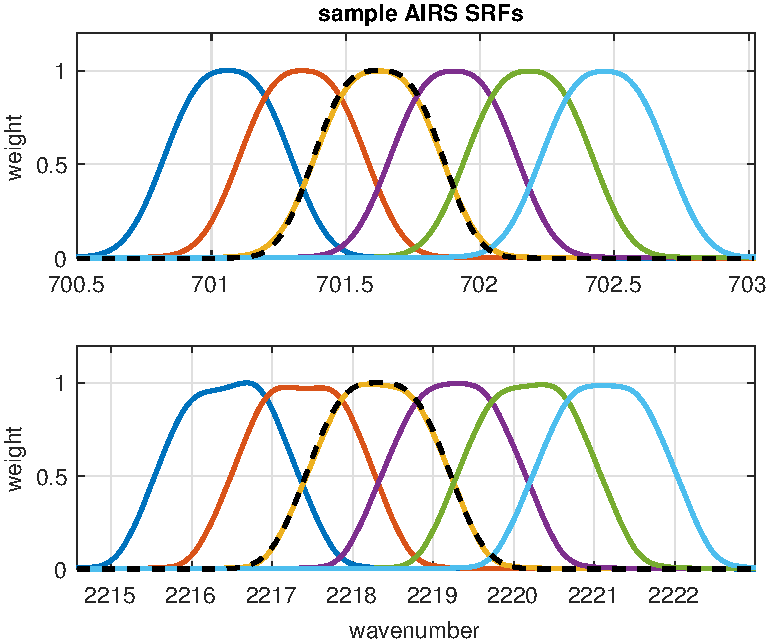
\includegraphics[width=\linewidth]{figures/airs_sample_SRF.pdf}
  \caption{sample {\airs} spectral response functions from the low
    and high ends of the band.   The dashed line is a generalized
    Gaussian function.}
  \label{srfs1}
\end{figure}

\begin{figure} % source plot_SRF2.m
  \centering
  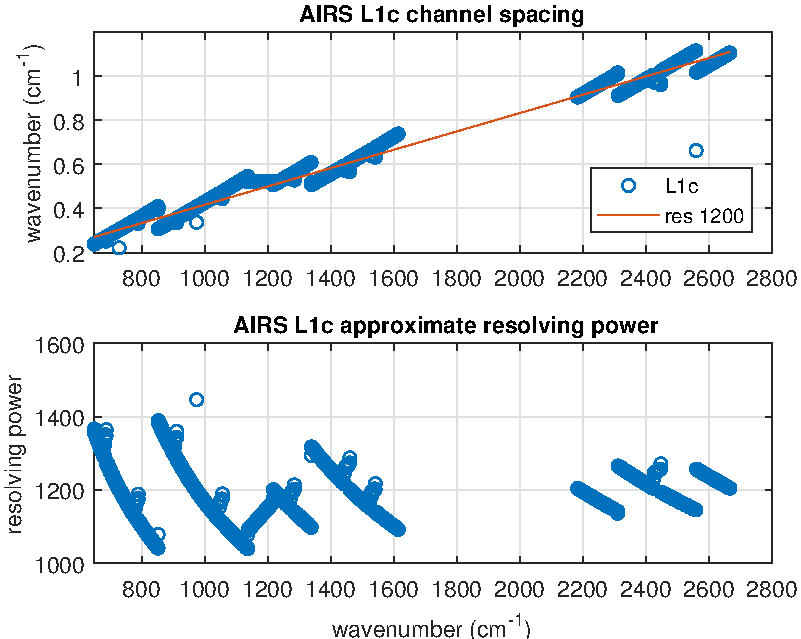
\includegraphics[width=\linewidth]{figures/airs_L1c_res.pdf}
  \caption{{\airs} L1c channel spacing and derived resolving
    power.}
  \label{chan1}
\end{figure}

Figure \ref{srfs1} shows typical {\airs} SRFs from the low and high
ends of the band.  Note the significant overlap in the wings.  This
can allow for a deconvolution to recover resolution beyond that of
the response functions considered individually.  The SRFs are not
necessarily symmetrical, especially at the high end of the band.
The dashed line on top of the third SRF in each group is a fit for a
generalized Gaussian, which we consider in more detail later in this
section.  Figure \ref{chan1} shows channel spacing and resolving
power for the {\airs} L1c channel set \cite{a1c:atbd}.  The variable
channel spacing and resolving power are due to the modular structure
of the focal plane.  Although not entirely regular---that is, not a
simple function of frequency---the L1c channel set is more regular
than the L1b channel set from which it is derived, and we mainly
consider the L1c set here.

Suppose we have $n$ channels and a frequency grid $\vec v$ of 
$k$ points spanning the union of the domains of the functions
$\sigma_i$.  The grid step size for our applications is often 0.0025
{\wn}, the default resolution for upwelling radiances calculated
with kcarta \cite{kcarta1}.  Let $S_k$ be an $n\times k$ array such 
that $s_{i,j} = \sigma_i(v_j)/w_i$, where $w_i = \sum_j \sigma_i(v_j)$,
that is where row $i$ is $\sigma_i(v)$ tabulated at the grid $\vec
v$ and normalized so the row sum is 1.  If the channel centers are
in increasing order $S_k$ is banded, and if they are not too close
(as is the case for a few of the L1b channels) the rows are linearly
independent.  $S_k$ is a linear transform whose domain is radiance
at the grid $\vec v$ and whose range is channel radiances.  If $r$
is radiance at the grid $\vec v$, then $c = S_k r$ gives a good
approximation of the channel radiances $c_i = \int\sigma_i(v)r(v)\,dv$.
In practice this is how we convolve kcarta or other high resolution
calculated radiances to get {\airs} channel radiances, for example
for reference truth or ``true {\airs}'' for the tests shown here.

% We construct $S_k$ either explicitly or implicitly from the
% {\airs} {\srf} tabulations.  The matrix $S_k$ in the former case
% is large but manageable with a banded or sparse representation.

For the {\airs} to {\cris} and other translations we are mainly
interested in the transform $S_b$ for {\srf}s at an intermediate
resolution, typically $0.1~\wn$.  This is the approximate resolution
of the {\srf} measurements and convenient for reconvolution to the
{\cris} user grid.  So let $\vec v_b = v_1,v_2,\ldots,v_m$ be a
$0.1~\wn$ grid spanning the domains of the functions $\sigma_i$.
Similar to $S_k$, let $S_b$ be an $n\times m$ array where row $i$ is
$\sigma_i(v)$ tabulated at the $\vec v_b$ grid, with rows normalized
to~1.  If $r$ is radiance at the $\vec v_b$ grid, then $c = S_b r$
is still a reasonable approximation of $\int\sigma_i(v)r(v)\,dv$.

For our application we want to start with $c$ and find $r$, that is
to deconvolve $c$ by solving $S_b r = c$ for $r$.  Since $m < k$ the
system is underdetermined.  We take the Moore-Penrose pseudoinverse
\cite{wiki:pinv} of $S_b$ to get $r_0 = S_b^{-1} c$.  This gives a
minimal solution, in the sense that $||r_0||_2 \le ||r_j||_2$ for
all $r_j$ satisfying $S_b r_j = c$.  The condition number for $S_b$
as built from the L1c channels is $||S_b||_2||S_b^{-1}||_2 = 115$,
which is tolerable.

Although our main goal is to reconvolve the $0.1~\wn$ intermediate
representation to the {\cris} or other user grids, we first compare
the deconvolved radiances with reference truth from a direct
convolution to the intermediate grid.  The choice of response
functions for the direct convolution is not obvious, since the
deconvolution is undoing---at least to some extent---the effects of
the {\airs} SRF convolutions.  We chose a generalized Gaussian 
\cite{wiki:gauss} of the form
\[w(v, v_0, \fwhm) = 
\exp\left(-\left(\frac{(v - v_0)^2}{2c^2}\right)^{1.5}\right) \]
where $c=\fwhm / (2\sqrt{2\ln 2})$ and $v_0$ is the desired channel
center.  The exponent $1.5$ was chosen to give an approximate match
to {\airs} SRFs with the same {\FWHM} and channel centers, though
without the fine structure and variation of the measured \srf s.
Figure \ref{srfs1} shows two such generalized Gaussians paired with
the corresponding {\airs} SRFs.  We used the same functions as
reference truth for the $0.1~\wn$ intermediate grid with ${\fwhm} =
v_i / 2000$, where $v_i$ are the grid frequencies.  This represents
a hypothetical grating spectrometer with a resolving power of 2000,
oversampled to the 0.1~\wn\ grid.  The value of 2000 was chosen to
give an approximate fit to the deconvolved radiances.  We also tried
a generalized Gaussian with a fixed {\FWHM} for values $0.4$, $0.6$,
and $0.8$ and a sinc basis with a spacing of $0.2$~\wn, all of which
gave larger residuals.

\begin{figure} % source decon_test1.m
  \centering
  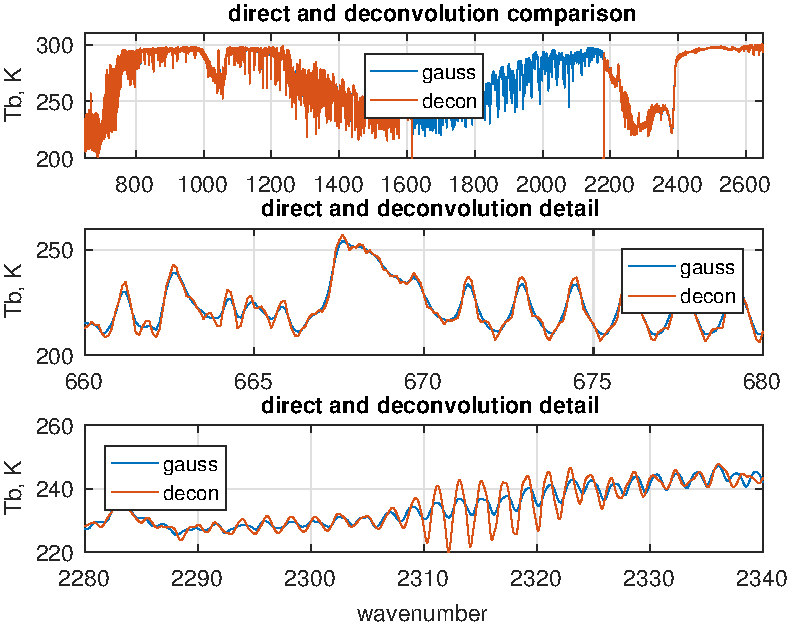
\includegraphics[width=\linewidth]{figures/airs_decon_spec.pdf}
  \caption{spectra from fitting profile 1 for direct convolution to
    the $0.1$~\wn\ grid (``gauss'') and deconvolved {\airs}}
  \label{dspec}
\end{figure}

\begin{figure} % source decon_test1.m 
  \centering
  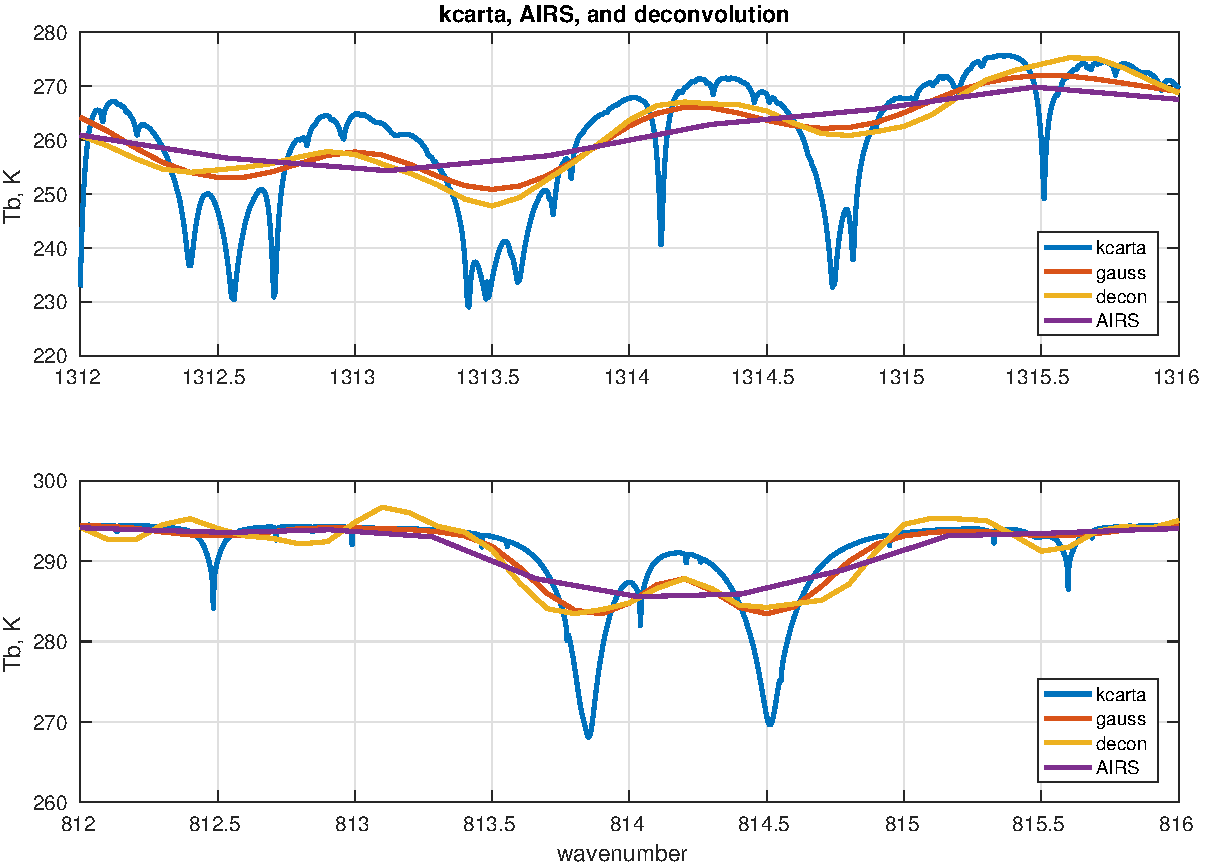
\includegraphics[width=\linewidth]{figures/airs_decon_zoom.pdf}
  \caption{details from fitting profile 1 for kcarta, direct
    convolution to the $0.1$~\wn\ grid (``gauss''), deconvolved
    {\airs}, and true {\airs}.}
  \label{dzoom}
\end{figure}

% \begin{figure} % source decon_test1.m
%   \centering
%   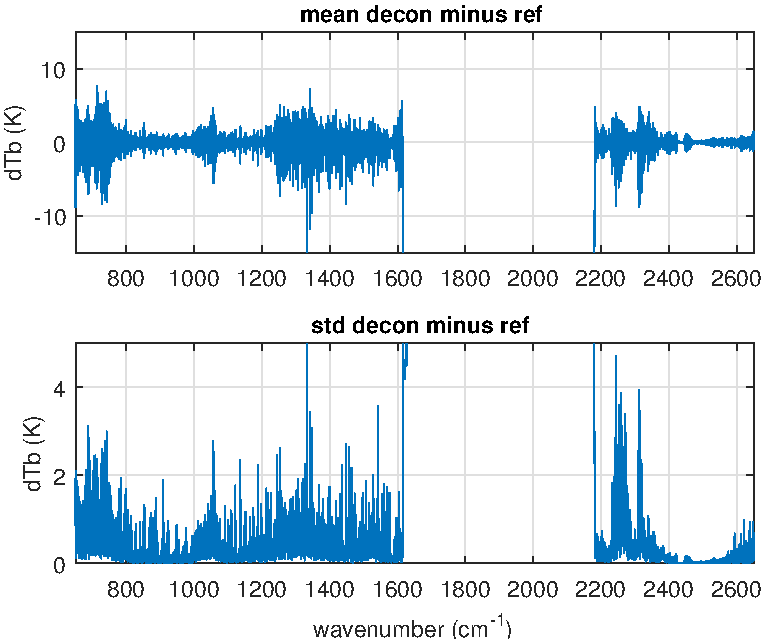
\includegraphics[width=\linewidth]{figures/airs_decon_diff.pdf}
%   \caption{mean and standard deviation over the 49 fitting profiles
%     for the L1c deconvolution minus direct convolution to the
%     $0.1$~\wn\ intermediate grid.  The residuals are too large to use
%     the deconvolved radiances directly.}
%   \label{ddiff}
% \end{figure}

The {\airs} deconvolution gives a modest resolution enhancement, at
the cost of added artifacts and noise.  Figure \ref{dspec} shows the
full spectra from fitting profile~1, along with sample details from
the low and high ends of the band, for the deconvolution and direct
convolution to the intermediate grid.  In the details we see some
overshoot and ringing in the deconvolution.  Figure \ref{dzoom}
shows details of kcarta, direct convolution to the $0.1$~\wn\ grid,
deconvolution, and AIRS spectra for fitting profile~1
\cite{sarta1,sarta2}.  In the first subplot we see the deconvolution
is capturing some of the fine structure in the kcarta data that is
present in the direct convolution but not in the AIRS data.  In the
second subplot we see the deconvolution (and direct convolution)
resolving a pair of close lines that are not resolved at the {\airs}
L1c resolution.  But we also see some ringing that is not present in
the direct convolution.  These artifacts are acceptable because we
do not propose using the deconvolved radiances directly; they are an
intermediate step before reconvolution to a lower resolution.

% Figure \ref{ddiff} shows the mean and standard deviation of the
% difference of the deconvolved minus the directly convolved radiances
% for all 49 fitting profiles.  The residuals are large but mainly
% significant for understanding limitations of the deconvolution.

% The residuals can be reduced dramatically by reconvolving the
% $0.1$~\wn\ intermediate grid to a lower resolution.  We consider
% this for convolution to the {\cris} user grid in the next section.

\begin{figure} % source plot_Binv.m
  \centering
  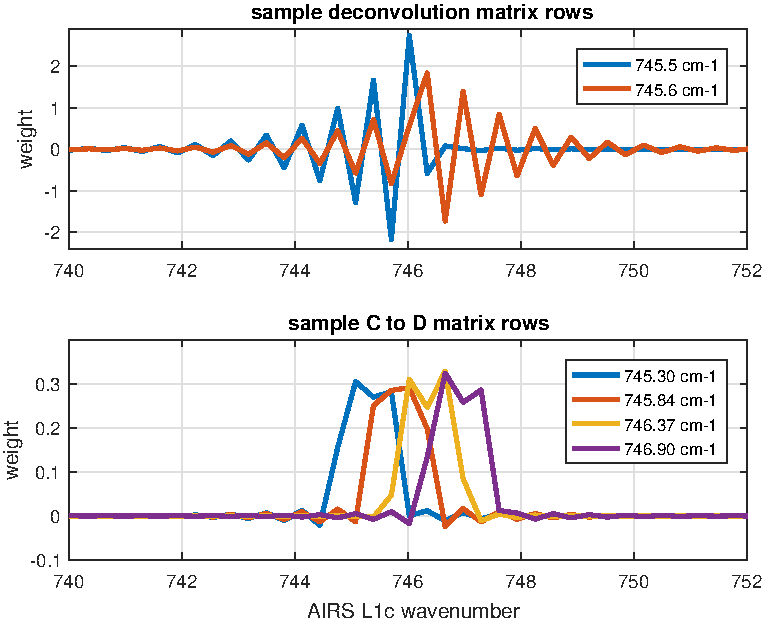
\includegraphics[width=\linewidth]{figures/airs_decon_basis.pdf}
  \caption{sample adjacent rows for the deconvolution and L1c to L1d
    transforms}
  \label{dbasis}
\end{figure}

Figure \ref{dbasis} shows a pair of typical adjacent rows of the
deconvolution matrix $S_b^{-1}$\, in the first subplot.  Row $i$ of
$S_b^{-1}$ is the weights applied to L1c channel radiances to
synthesize the deconvolved radiance $r_i$ at the intermediate grid
frequency $v_i$.  The oscillation shows we are taking the closest
AIRS channel, subtracting weighted values for channels $\pm 1$ step
away, adding weighted values for channels $\pm 2$ steps away, and so
on, with the weights decreasing quickly as we move away from $v_i$,
with eight to ten L1c channels making a significant contribution to
each deconvolution grid point.  The second subplot shows four
adjacent rows of the matrix $S_d \cdot S_b^{-1}$, which takes L1c to
L1d channel radiances.  (The L1d radiances are discussed in a later
section; here they are of interest mainly as a typical
reconvolution.)  Both matrices are banded but the bands are narrower
in the second, with three to five L1c channels contributing
significantly to each L1d channel.  The range of influence is
significant since we may want to know which L1d channels are derived
in part from the synthetic L1c channels.

%---------------------------------------------------------------------
\FloatBarrier
\section{AIRS to CrIS translation}
\label{airs2cris}

Given {\airs} deconvolution to a $0.1~\wn$ intermediate grid,
reconvolution to the {\cris} user grid is straightforward.  For the
{\cris} standard resolution the channel spacing is $0.625~\wn$ for
the LW band, $1.25~\wn$ for the MW, and $2.5~\wn$ for the SW.  
For each {\cris} band, we (1) find the {\airs} and {\cris} band
intersection, (2) apply a bandpass filter to the deconvolved {\airs}
radiances restricting them to the intersection, with a rolloff
outside the intersection, and (3) reconvolve the filtered spectra to
the {\cris} user grid with a zero-filled double Fourier transform
\cite{git:finterp}.

Translations are tested by comparison with calculated reference
truth.  We start with a set of atmospheric profiles and calculate
upwelling radiance at a $0.0025~\wn$ grid with kcarta \cite{kcarta1}
over a band spanning the domains of the {\airs} and {\cris} response
functions.  ``True {\airs}'' is calculated by convolving the kcarta
radiances with {\airs} SRFs and ``true {\cris}'' by convolving
kcarta radiances to a sinc basis at the {\cris} user grid.  True
{\airs} is then translated to {\cris} to get ``{\airs} {\cris}'',
and this is compared with true {\cris}.  Figure~\ref{specLW} shows
sample spectra for true {\airs}, deconvolved {\airs}, true {\cris}
and {\airs} {\cris}.  The difference between true {\cris} and
{\airs} {\cris} is hard to see at this level of detail, and for the
remainder of this paper we will mainly show explicit differences.

For most tests we use a set of 49 fitting profiles spanning a wide
range of clear atmospheric conditions, initially chosen for testing
radiative transfer codes \cite{sarta1,sarta2}.  The set is largely
uncorrelated; reducing the reconstruction residual to 0.02~K
requires 48 left-singular vectors.  (Details of this correlation
measure are given in an appendix.)  For statistical correction and
the direct regression discussed in section \ref{dregr} we also use a
set of 7377 radiances calculated from all-sky (clear and cloudy)
AIRS profiles spanning several consecutive days as the dependent
set.  This set is moderately correlated; reducing the reconstruction
residual to 0.02~K requires 260 left-singular vectors.  Splitting
the 7377 profile set into dependent and independent subsets and
comparing residuals from the independent subset with residuals from
the 49-profile set, we found residuals from the latter are
consistently larger, suggesting it makes for a stricter test.  So
for the results shown here the test or independent set is always the
49-profile set, while for tests requiring fitting the 7377 profile
is used as the dependent set.

Figures \ref{diffLW}, \ref{diffMW}, and \ref{diffSW} show the mean
and standard deviation of true {\cris} minus {\airs} {\cris} for the
49 fitting profiles, with and without Hamming apodization, for each
of the {\cris} bands.  Figure \ref{meanAll} summarizes these results
for Hamming apodized radiances.  The residual has a high frequency
component with a period of 2 channel steps that is significantly
reduced by the apodization.  The constant or DC bias is very close
to zero for the apodized residuals.

% $0.002$~K for the LW, $-0.005$~K for the MW, and $0.001$~K for the
% SW.

\begin{figure} % source a2cris_test1
  \centering
  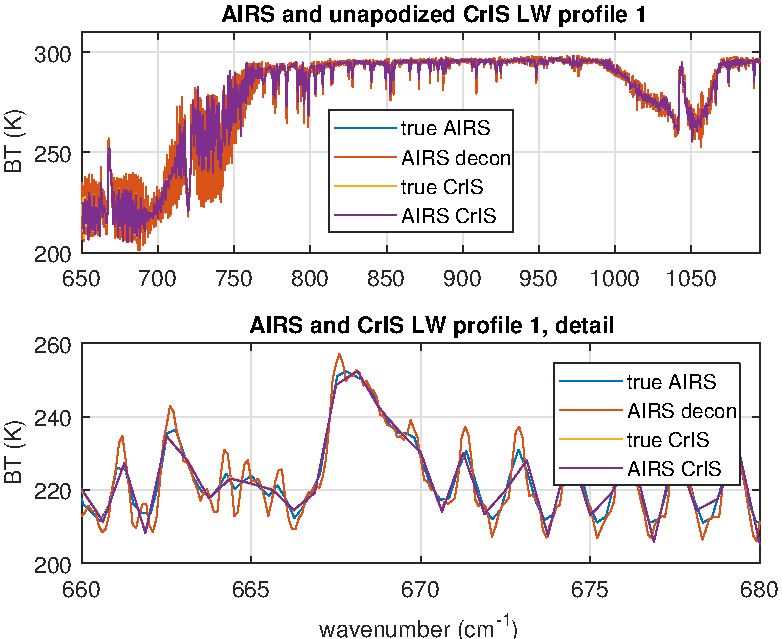
\includegraphics[width=\linewidth]{figures/a2cris_spec_LW.pdf}
  \caption{true {\airs}, deconvolved {\airs}, true {\cris}, and {\airs}
    {\cris}.  Differences between true {\cris} and {\airs} {\cris} are too
    small to be visible in this figure.}
  \label{specLW}
\end{figure}

\begin{figure} % source a2cris_test1
  \centering
  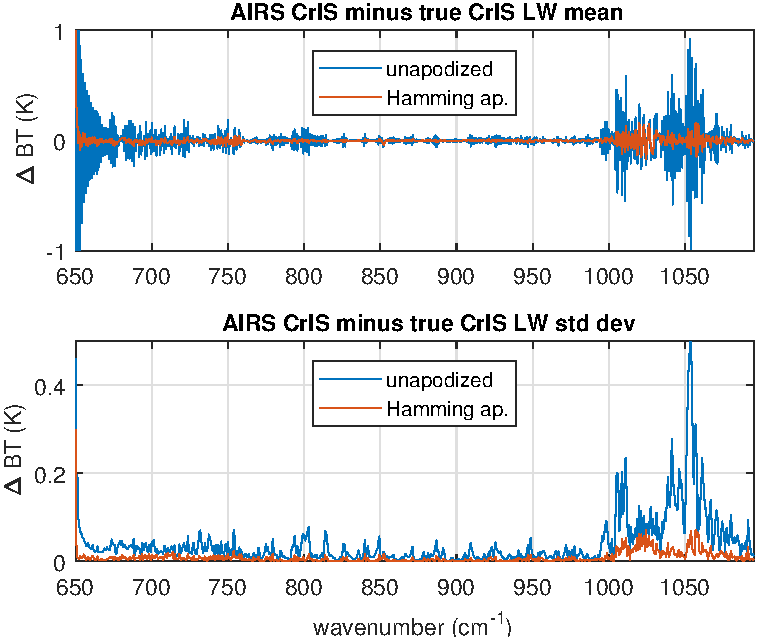
\includegraphics[width=\linewidth]{figures/a2cris_diff_LW.pdf}
  \caption{Mean and standard deviation of unapodized and Hamming
    apodized {\airs} {\cris} minus true {\cris}, for the {\cris} LW
    band}
  \label{diffLW}
\end{figure}

\begin{figure} % source a2cris_test1
  \centering
  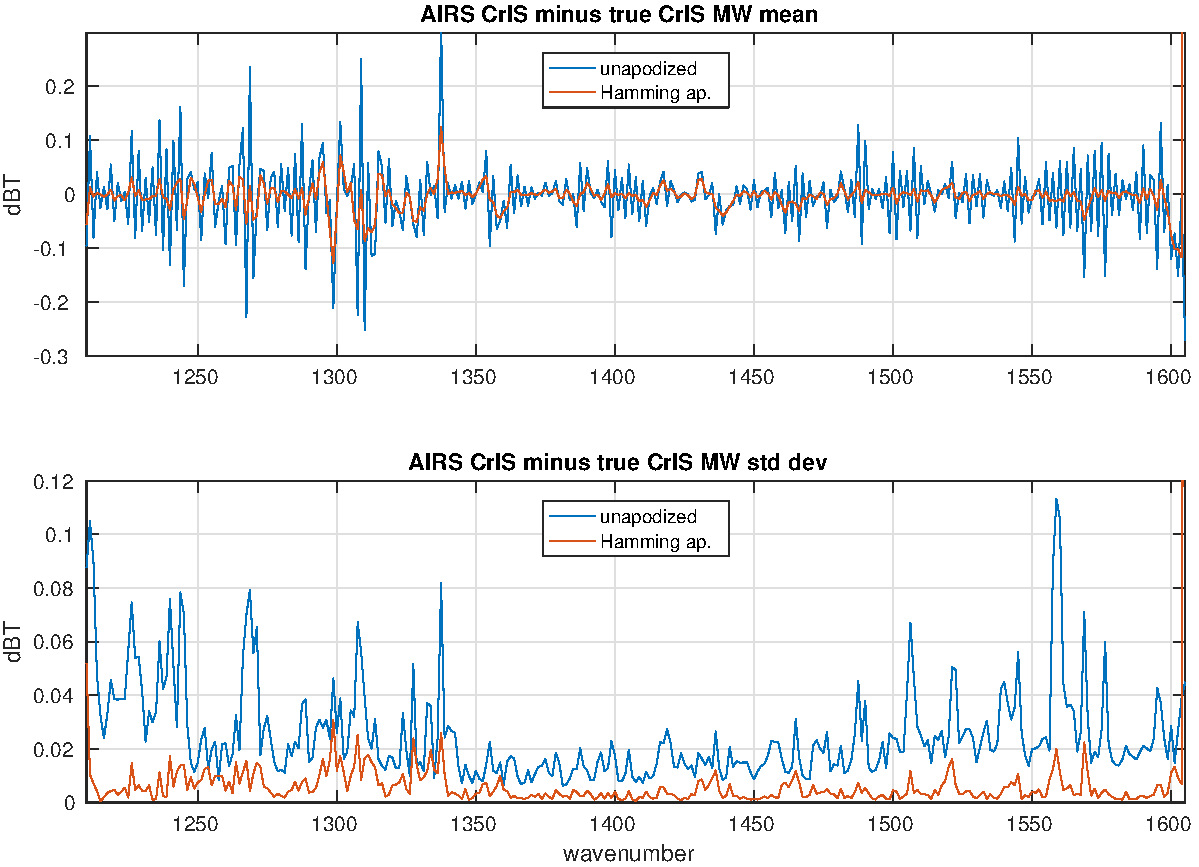
\includegraphics[width=\linewidth]{figures/a2cris_diff_MW.pdf}
  \caption{Mean and standard deviation of unapodized and Hamming
    apodized {\airs} {\cris} minus true {\cris}, for the {\cris} MW
    band}
  \label{diffMW}
\end{figure}

\begin{figure} % source a2cris_test1
  \centering
  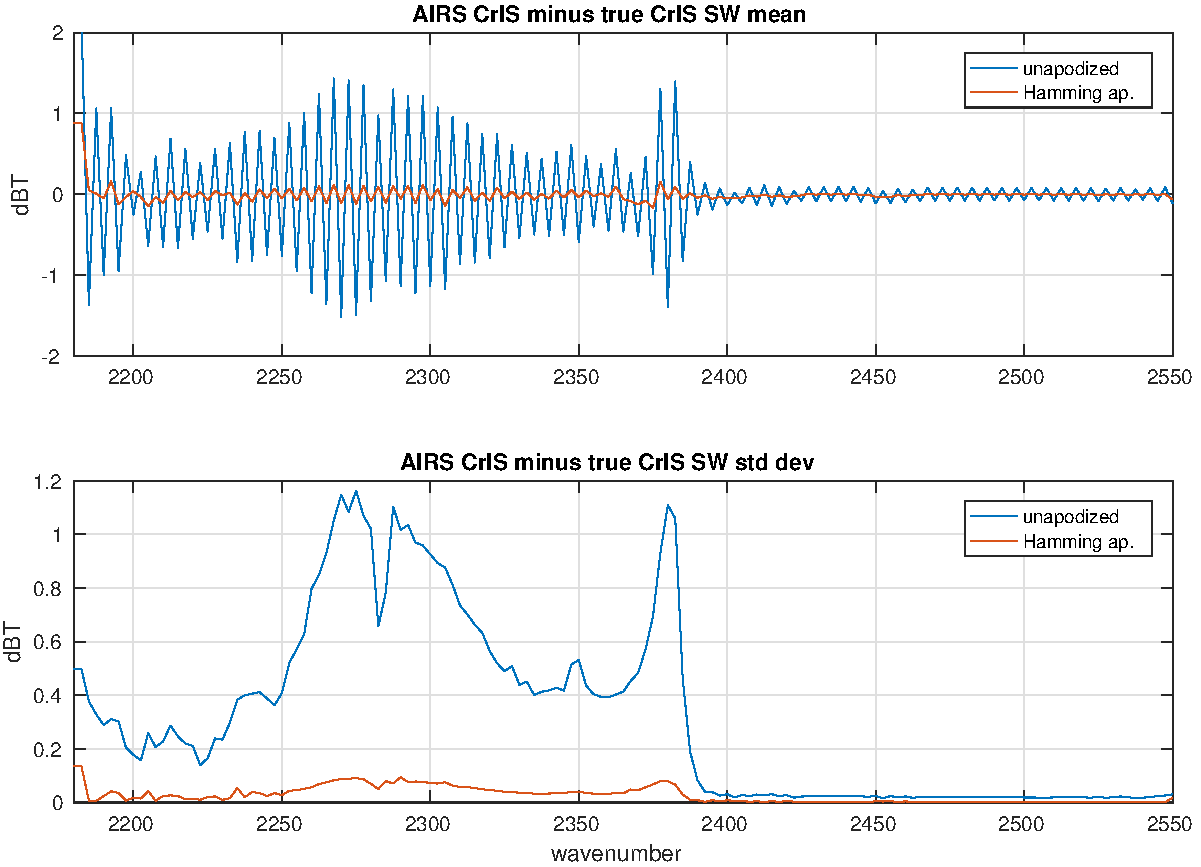
\includegraphics[width=\linewidth]{figures/a2cris_diff_SW.pdf}
  \caption{Mean and standard deviation of unapodized and Hamming
    apodized {\airs} {\cris} minus true {\cris}, for the {\cris} SW
    band}
  \label{diffSW}
\end{figure}

\begin{figure} % source a2cris_test1
  \centering
  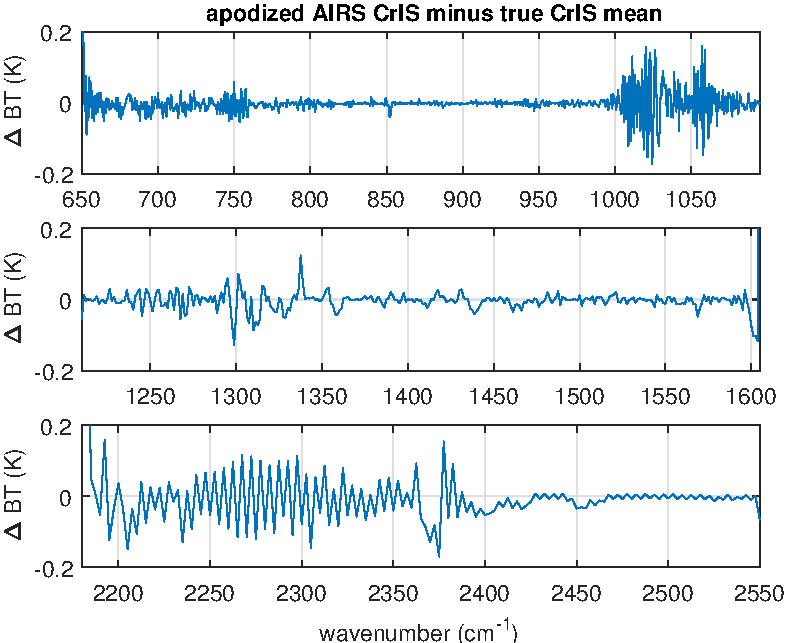
\includegraphics[width=\linewidth]{figures/a2cris_diff_all.pdf}
  \caption{Mean of apodized residuals for all three {\cris} bands}
  \label{meanAll}
\end{figure}

Some regularity remains in the apodized residual, including the
oscillation with a period of two channel steps.  Up to this point
there as been no statistical component to our translation, beyond
the choice of test set for validation.  We feel it is important to
be clear about any steps that require statistical fitting.  That
said, a simple linear correction can give a significantly further
reduction of the residuals.  For such tests as noted we use the set
of 7377 mostly cloudy AIRS profiles as the dependent set and the 49
profile set the independent or test set.

We compare three such corrections.  These are done with a separate
regression for each {\cris} channel, and so introduce no
cross-correlations.  Let $\Ttc_i$ be true {\cris} and $\Tac_i$
{\airs} {\cris} brightness temperatures for {\cris} channel $i$,
from the dependent set.  For the bias test we subtract the mean
residual from the dependent set.  For the linear test we find $a_i$
and $b_i$ to minimize $||a_i\,\Tac_i + b_i - \Ttc_i||_2$, and for
the quadratic test weights $c_i$, $a_i$ and $b_i$ to minimize
$||c_i\,(\Tac_i)^2 + a_i\,\Tac_i + b_i - \Ttc_i||_2$.  The resulting
correction is then applied to the independent set, the 49 fitting
profiles, for comparison with true {\cris}.

Figure \ref{statLW} is a comparison of bias, linear, and quadratic
corrections for the LW band.  The linear and quadratic corrections
are nearly identical, and the quadratic coefficient is very close to
zero.  Figure \ref{coefLW} shows the weights for the linear fits
from figure \ref{statLW}.  The $a$ weights are very close to 1 and
the $b$ weight to the bias.  Figures \ref{statMW} and \ref{statSW}
show the linear correction giving a similar improvement in the MW
and a small improvement in the SW, where the quadratic correction is
noticably worse.  Figure \ref{statAll1} shows the residuals for the
apodized linear correction for all three bands.  The residuals are
significantly reduced in comparison with the apodized uncorrected
radiances shown in figure \ref{meanAll}.

% Note that convolution, deconvolution, and apodization are done
% with radiances while spectra are presented and statistics done
% after translation to brightness temperatures.

\begin{figure} % source a2cris_regr2.m
  \centering
  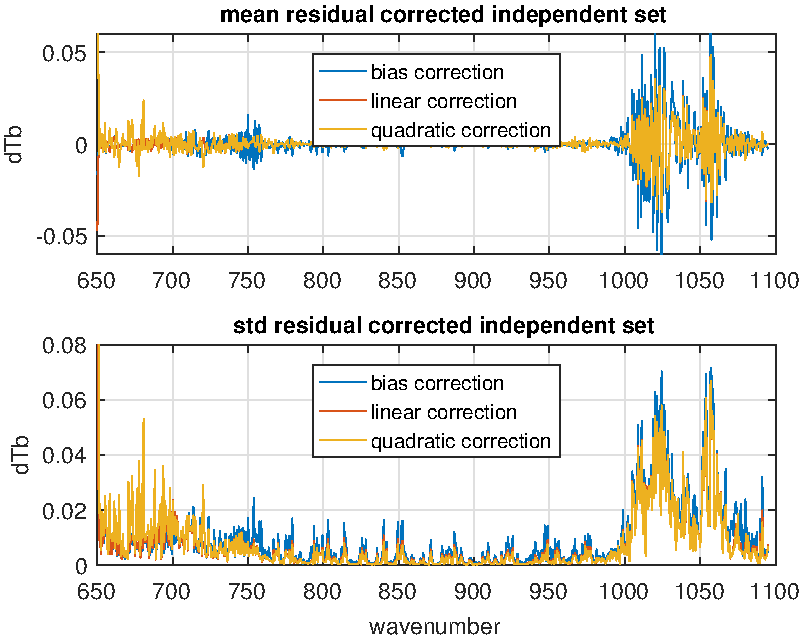
\includegraphics[width=\linewidth]{figures/a2cris_regr_LW.pdf}
  \caption{Mean and standard deviation of LW corrected apodized
    residuals}
  \label{statLW}
\end{figure}

\begin{figure} % source a2cris_regr2.m
  \centering
  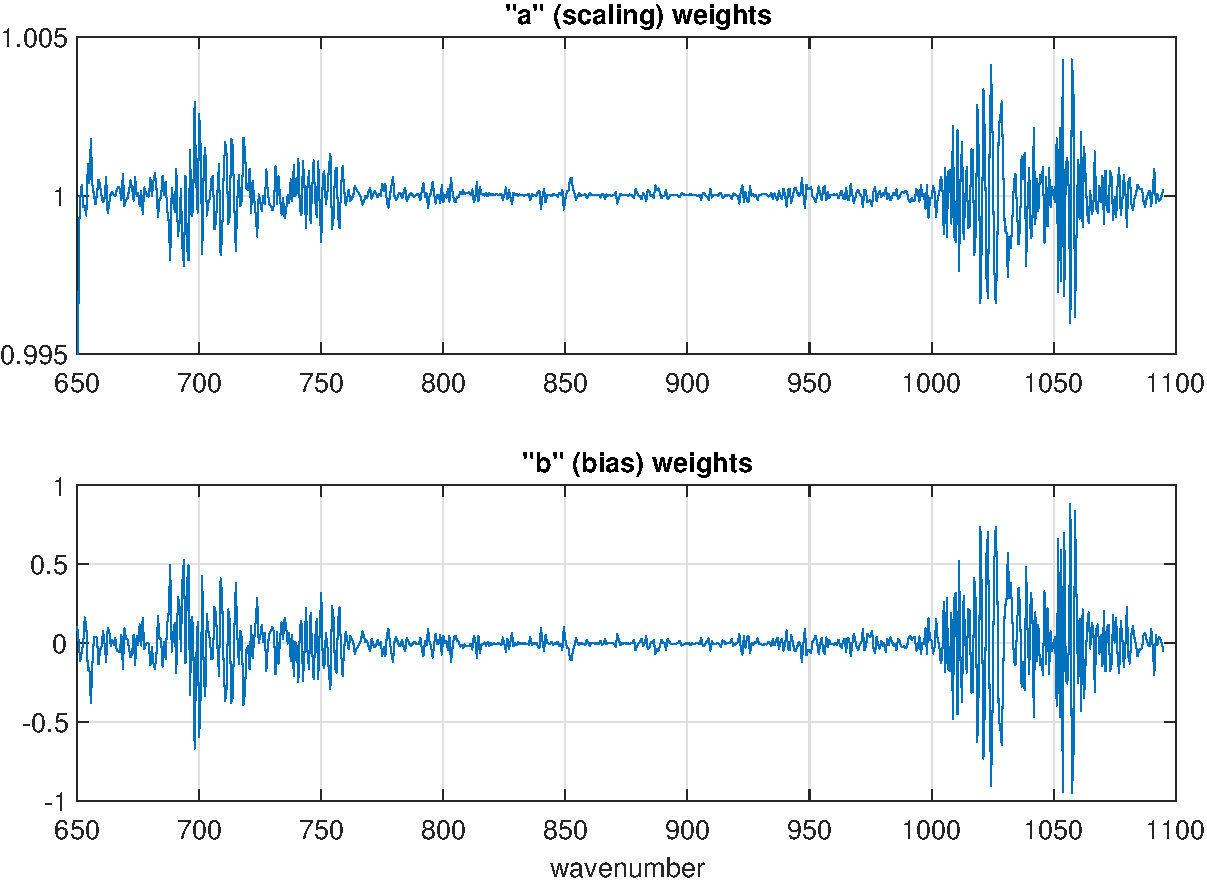
\includegraphics[width=\linewidth]{figures/a2cris_coef_LW.pdf}
  \caption{LW $a$ and $b$ weights for the linear correction $ax+b$}
  \label{coefLW}
\end{figure}

\begin{figure} % source a2cris_regr2.m
  \centering
  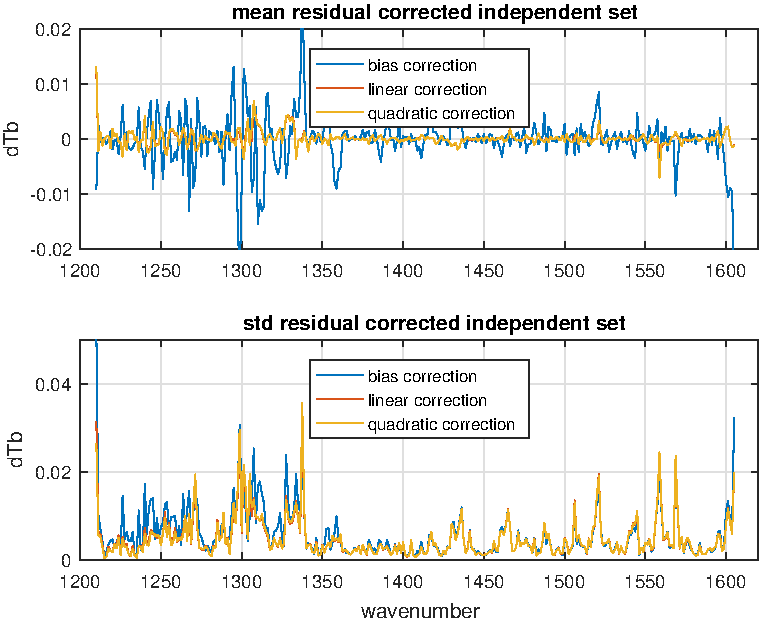
\includegraphics[width=\linewidth]{figures/a2cris_regr_MW.pdf}
  \caption{Mean and standard deviation of MW corrected apodized
    residuals.}
  \label{statMW}
\end{figure}

\begin{figure} % source a2cris_regr2.m
  \centering
  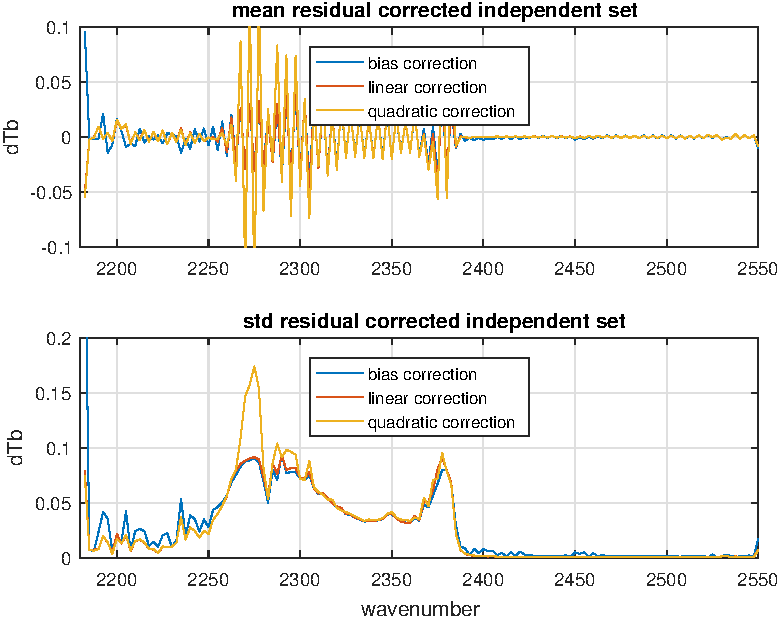
\includegraphics[width=\linewidth]{figures/a2cris_regr_SW.pdf}
  \caption{Mean and standard deviation of SW corrected apodized
    residuals.}
  \label{statSW}
\end{figure}

\begin{figure} % source a2cris_test2.m
  \centering
  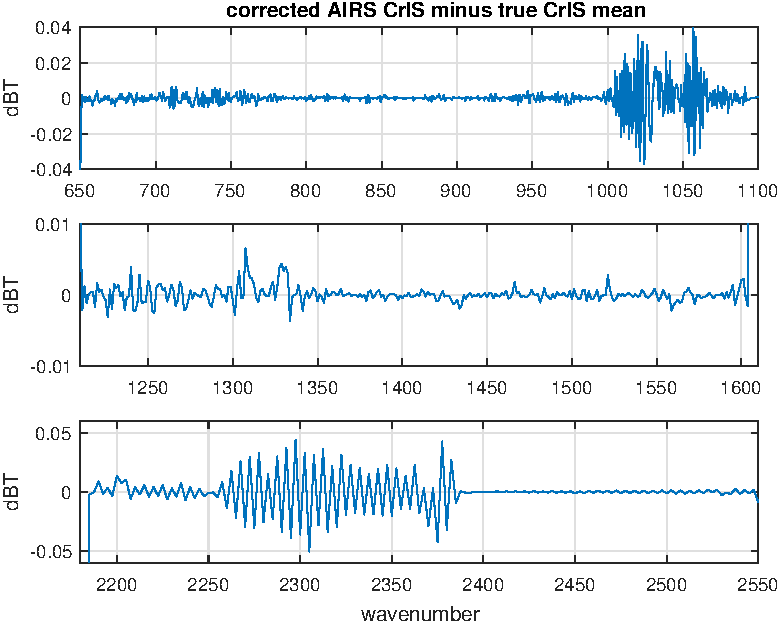
\includegraphics[width=\linewidth]{figures/ap_decon_corr.pdf}
  \caption{Mean corrected apodized residuals for all three bands.}
  \label{statAll1}
\end{figure}

% \begin{figure} % source a2cris_test2.m
%   \centering
%   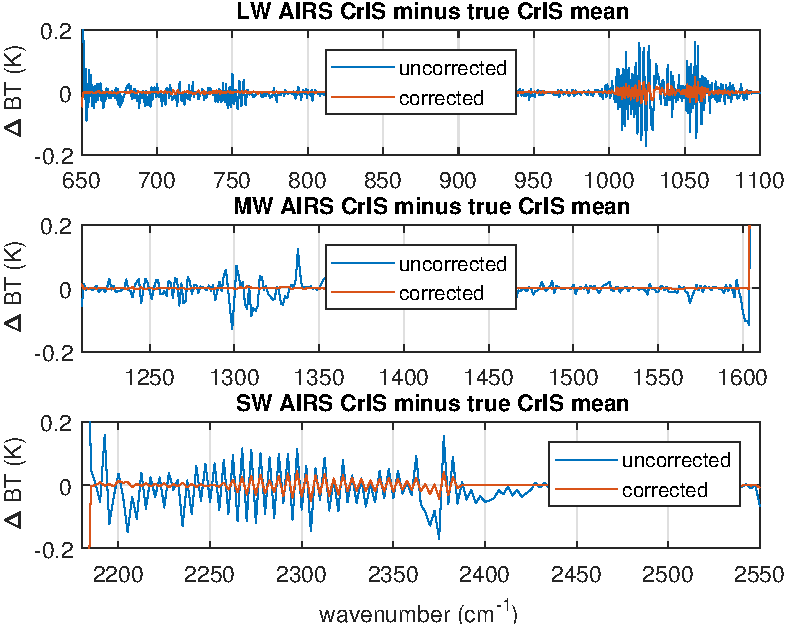
\includegraphics[width=\linewidth]{figures/a2cris_regr_all.pdf}
%   \caption{Mean corrected and uncorrected apodized residuals for all
%     three bands.}
%   \label{statAll2}
% \end{figure}

We can give a good estimate of noise equivalent differential
radiance (NEdN) for the translation by adding noise with a normal
distribution at the {\airs} NEdN spec to blackbody radiance at 280K
and translating this to {\cris}.  This is done repeatedly and the
noise after translation is measured.  As a check, noise before
translation is also measured and compared with the {\airs} value.
Figure \ref{nedn} shows this measured {\airs}-to-{\cris} together
with {\airs} and {\cris} NEdN for both apodized and unapodized
radiances.  The {\airs} and {\cris} values are averages over a full
day, 4 Dec 2016.  NEdN for the L1c synthetic channels is
interpolated.  The first subplot of figure \ref{nedt} is NEdT for
apodized radiances, for fitting profile 1.

The {\airs} channel-to-channel NEdN variation is significant; in the
upper half of the LW and most of the MW it is of the same order as
the {\airs} and {\cris} NEdN difference.  This variation is due the
{\airs} focal plane structure and sensitivity.  The {\airs} and
{\cris} NEdN measures are both spiky when averaged over a few
minutes but the {\cris} variation is primarily uncertainty in the
noise measurement and smooths out as the time span is extended
while the {\airs} variation is stable.  The {\airs}-to-{\cris}
translation inherits this variability; it is a significant part of
the difference between {\airs} {\cris} and true {\cris}.  For a
common record we might want to add noise on a channel-by-channel
basis to whichever NEdN value---{\airs} {\cris} or true {\cris}---is
lower.  NEdN for the combined record would then be max of the
{\airs} {\cris} and true {\cris} NEdN values, as shown in the second
subplot of figure \ref{nedt}.

\begin{figure} % source nedn_test2.m
  \centering
  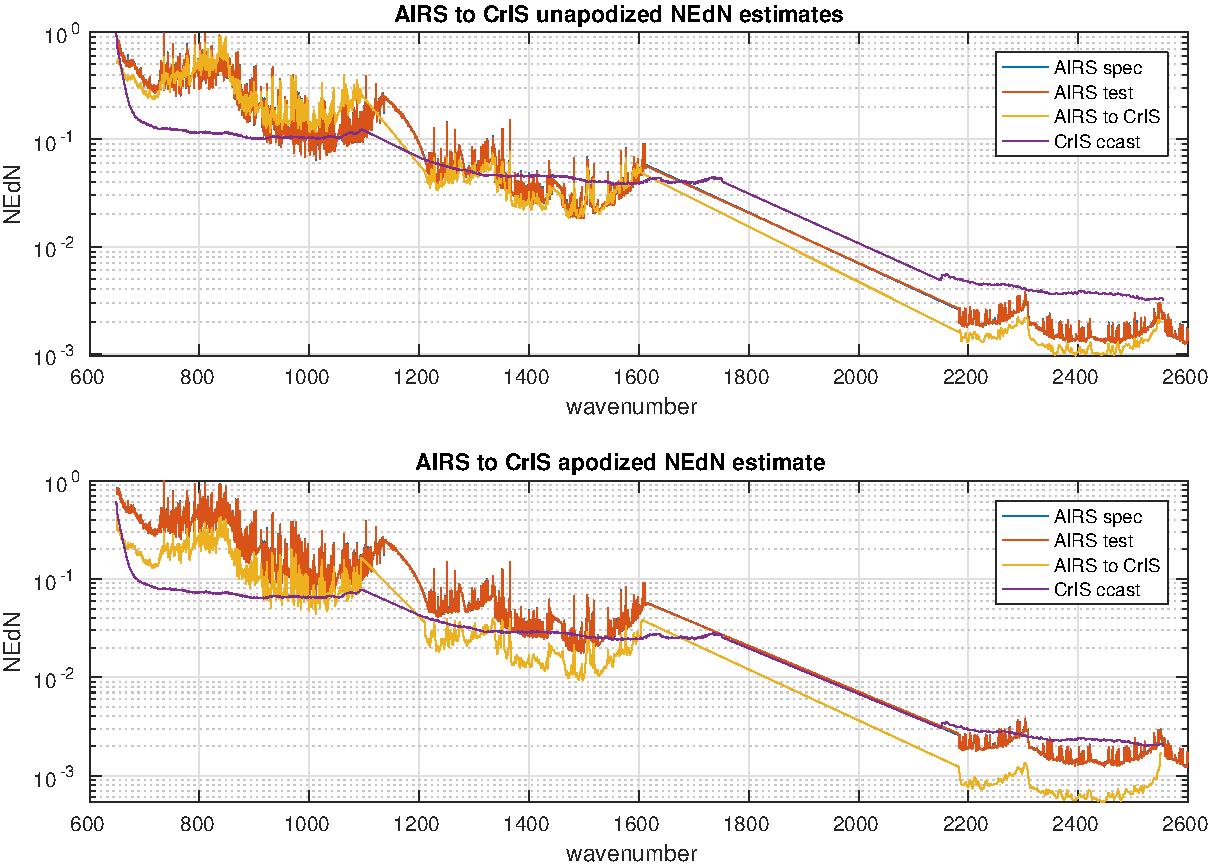
\includegraphics[width=\linewidth]{figures/a2cris_nedn.pdf}
  \caption{mean {\airs}, {\airs}-to-{\cris}, and mean {\cris}
    apodized and unapodized NEdN.}
  \label{nedn}
\end{figure}

\begin{figure} % source nedt_test1.m
  \centering
  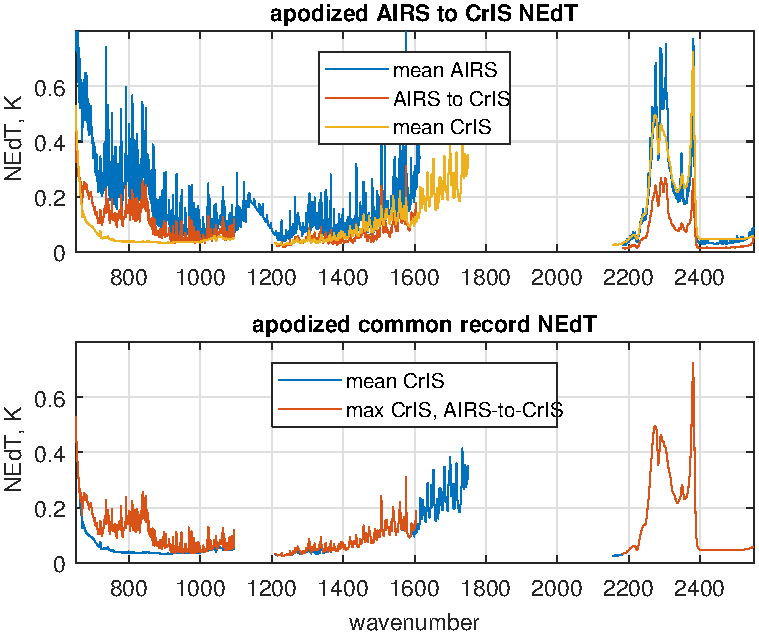
\includegraphics[width=\linewidth]{figures/a2cris_nedt.pdf}
  \caption{{\airs}, {\airs}-to-{\cris}, and {\cris} apodized NEdT,
    and the max of {\cris} and {\airs}-to-{\cris} with {\cris}
    NEdN shown as a reference.}
  \label{nedt}
\end{figure}

The {\airs} to {\cris} translation via deconvolution works
significantly better than conventional interpolation.  We consider
two cases.  For the first, start with true {\airs} and interpolate
radiances directly to the {\cris} user grid with a cubic spline.
For the second, interpolate true {\airs} to the 0.1 {\wn}
intermediate grid with a cubic spline and then convolve this to the
use {\cris} user grid.  Figure~\ref{intpLW} shows interpolated
{\cris} minus true {\cris} for the LW band, without apodization.
The two-step interpolation works a little better than the simple
spline, but both residuals are significantly larger than for the
translation with deconvolution.  Results for the MW are similar,
while the unapodized comparison is less clear for the SW.  With
Hamming apodization, the residuals with deconvolution are
significantly less than interpolation for all three bands.

\begin{figure} % source a2cris_test1
  \centering
  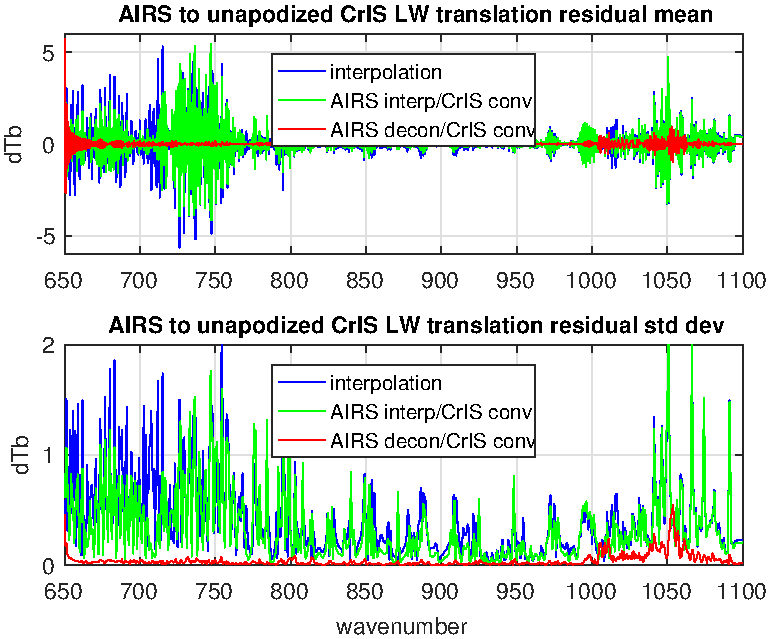
\includegraphics[width=\linewidth]{figures/a2cris_interp_LW.pdf}
  \caption{spline interpolation, interpolation with convolution, 
    and deconvolution with convolution for the {\cris} LW band.}
  \label{intpLW}
\end{figure}

%---------------------------------------------------------------------
\FloatBarrier
\section{Translation to an idealized grating model}
\label{airsL1d}

% The nominal {\airs} resolution is 1200, though for many modules
% the real resolving power is higher.

The {\airs} deconvolution can be used for other translations.  
In this section we briefly consider reconvolution to an idealized
grating model for resolving powers of 700 and 1200.  Define an
{\airs} L1d basis with resolving power $R$ using the generalized
Gaussian response function of section \ref{decon} as follows.
Let $v_0$ be the frequency of the first channel and for $i\ge0$
$\fwhm_i = v_i / R$, $dv_i = \fwhm_i / 2$, and $v_{i+1} = v_i +
dv_i$.  As with tests of the {\airs} to {\cris} translation, true
L1c is calculated by convolving kcarta radiances with {\airs} L1c
SRFs and true L1d by convolving with an L1d basis at the desired
resolving power.  L1c is translated to L1d by deconvolution followed
by reconvolution to the desired L1d basis, and this is compared with
true L1d.

Figure \ref{L1d1200} shows residuals for reconvolution to an L1d
basis with resolving power of 1200, the nominal {\airs} resolution,
and figure \ref{L1d700s} shows residuals for a resolving power of
700.  Note the different x-axes for the two figures.  The residuals
depend in part on the L1d starting channel $v_0$, and so on how the
L1c and L1d SRF peaks line up.  The residuals shown are the result
of a rough fit for $v_0$.  For a resolving power of 1200 this gave
$v_0$ equal to the first L1c channel, while for 700 it was the first
L1c channel plus $0.2$~\wn.

We see that for both the {\airs} to {\cris} and L1c to L1d
translations some resolving power is sacrificed in shifting channel
centers to a single regular function of frequency.  Residuals for a
resolving power of 1200 (figure \ref{L1d1200}) are roughly
comparable to unapodized {\cris} (figures \ref{diffLW},
\ref{diffMW}, and \ref{diffSW}) and residuals for a resolving power
of 700 (figure \ref{L1d700s}) are roughly comparable to apodized
{\cris} (figure \ref{statAll1}).  As with the {\airs} to {\cris}
translation, the L1c to L1d residuals are significantly reduced with
a linear correction.  Residuals for L1d with a resolving power of
700 after correction are comparable to residuals for apodized
{\cris} after a similar correction.

\begin{figure} % source L1d_regr1.m
  \centering
  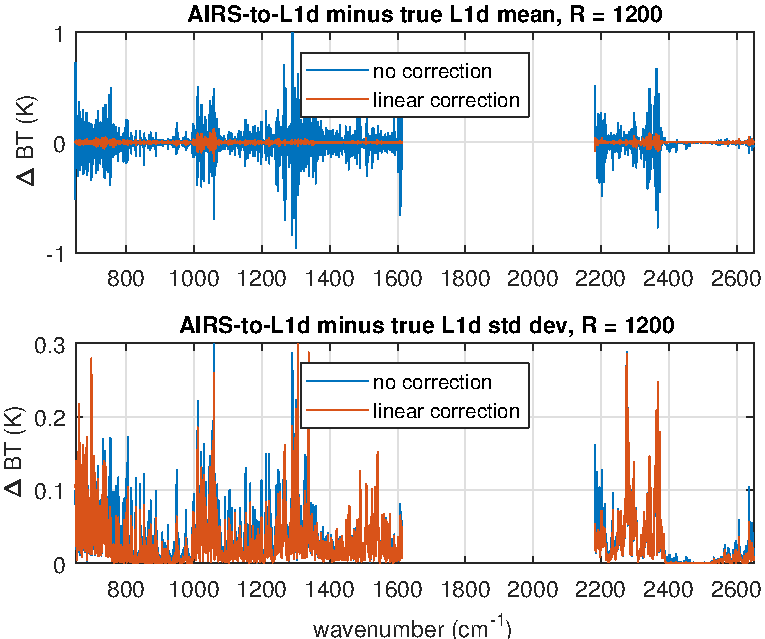
\includegraphics[width=\linewidth]{figures/L1d_cor1_1200.pdf}
  \caption{mean and standard deviation over the 49 fitting profiles
    for the L1c to L1d translation minus true L1d for a resolving
    power of 1200}
  \label{L1d1200}
\end{figure}

\begin{figure} % source L1d_regr1.m
  \centering
  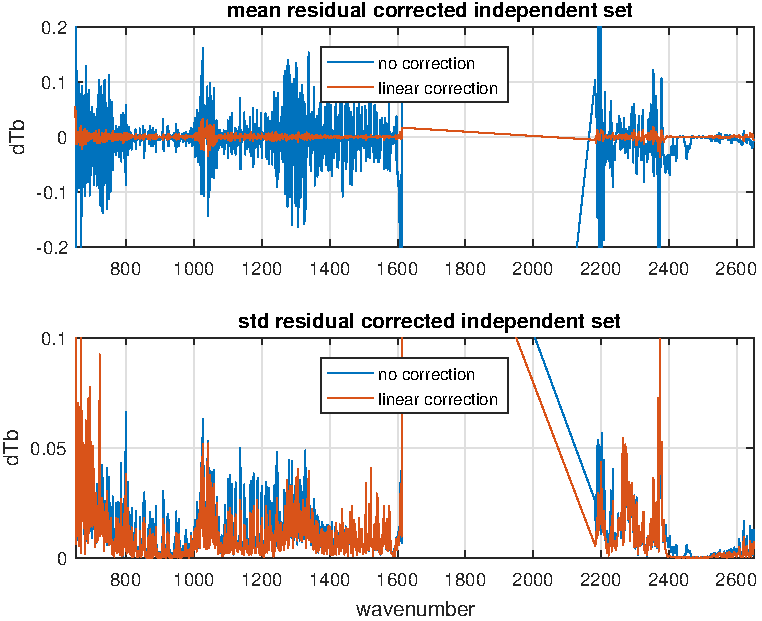
\includegraphics[width=\linewidth]{figures/L1d_cor1_700.pdf}
  \caption{mean and standard deviation over the 49 fitting profiles
    for the L1c to L1d translation minus true L1d for a resolving
    power of 700}
  \label{L1d700s}
\end{figure}

As with the {\airs} to {\cris} translation, deconvolution works
significantly better than interpolation.  We consider similar cases.
For the first, start with true L1c and interpolate radiances
directly to the L1d grid with a cubic spline.  For the second,
interpolate true L1c to the 0.1 {\wn} intermediate grid with a cubic
spline and convolve this to the L1d channel set.
Figure~\ref{interpL1d} shows interpolated L1d minus true L1d.  The
two-step interpolation works a little better than the simple spline,
but is still much larger than the residual for translation with
deconvolution.

\begin{figure} % source L1d_test2.m
  \centering
  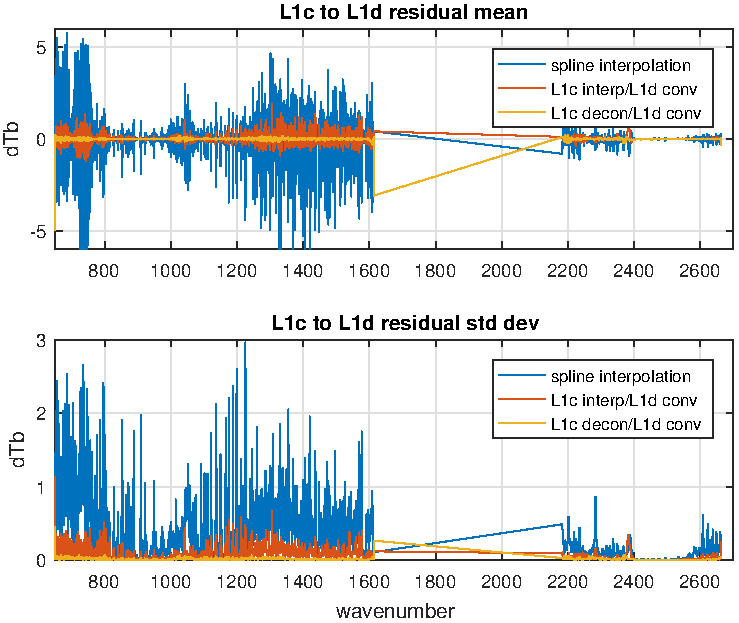
\includegraphics[width=\linewidth]{figures/CtoD_interp_diff.pdf}
  \caption{spline interpolation, interpolation with convolution, 
    and deconvolution with convolution for the {\airs} L1c to L1d
    translation with $v_0=649.822$~\wn\ and a resolving power of 700}
  \label{interpL1d}
\end{figure}

%---------------------------------------------------------------------
\FloatBarrier
\section{Principal component regression}
\label{dregr}

The {\airs} L1c to L1d translation can be done with a single linear
transform $S_d\cdot S_c^{-1}$, where $S_c$ and $S_d$ are the
transforms taking the intermediate grid to L1c and L1d channels.
The {\airs} to {\cris} translation can also be done with a composite
transform if we use a resampling matrix rather than the double
Fourier interpolation to go from the intermediate grid to the {\cris}
user grid.  We can get such a one-step tranform in other ways.  For
example if $r_a$ and $r_c$ are $m \times k$ and $n \times k$ {\airs}
and {\cris} radiance sets, we can find $X$ to minimize $\|X r_a -
r_c\|_2$.  Typically $k > m$, giving an overdetermined system, and
we solve $r_a^t X^t = r_c^t$ for $X$ by regression.  This is
different from the corrections of section \ref{airs2cris} and
\ref{airsL1d}; there regression was used to find linear or quadratic
correction coefficients independently for each channel.

Figures \ref{dreg1} shows residuals for direct regression, for
apodized radiances.  As before we use the 7377 profile set as the
dependent and the 49 profile as the independent sets.  The residuals
are roughly comparable to the residuals from the deconvolution
translation summarized in figure \ref{statAll1}.  The LW residual is
larger at the low end of the band for direct regression and the high
end for the deconvolved translation.  Deconvolution does better in
the MW, and direct regression in the SW.   Unfortunately the
regression matrices show significant off-diagonal correlations.
Figure \ref{dreg3} shows this for the LW; the MW and SW bands are
worse.  As noted in section \ref{airs2cris} the 7377 profile
dependent set is highly correlated.  The effective dimension is only
260, our regression is actually under-determined.  The dependent set
residuals are close to zero, much less than the residuals for the
independent set shown above.

One fix is to add noise.  Recall that we generate true {\airs} 
and true {\cris} by convolving a common set of high-resolution
radiances.  For true {\airs} we can simply add noise at the {\airs}
NEdN spec.  But for regression or testing of an {\airs} to {\cris}
translation we want {\cris} radiances with actual translated {\airs}
noise, not simply true {\cris} with noise added as per the {\cris}
NEdN spec.  The latter does reduce correlations but increases
residuals for the independent set significantly.

To model NEdN for the AIRS to CrIS translation we synthesize noise
at the {\airs} NEdN spec, add it to the signal, run it through the
translation, and measure it.  That works fine for measuring noise.
But to get an {\airs} to {\cris} translation by regression with
added noise we need the reference translation of each noisy {\airs}
spectra.  One way to do that might be to add noise to the high res
spectra before convolution to the {\airs} user grid in such a way
that we match the {\airs} NEdN spec and convolve this noisy signal
to the {\cris} user grid to get noisy {\cris}, but we do not pursue
that further here.

As an alternative to adding noise, we can use a form of principal
component regression.  As above, let $r_a$ and $r_c$ be $m \times k$
and $n \times k$ {\airs} and {\cris} radiance sets.  Let $r_a = U_a
S_a\,V_a^T$ be the singular value decomposition with singular values
in descending order and $U_a^i$ the first $i$ columns of $U_a$.
Similarly let $r_c = U_c S_c\,V_c^T$ be a singular value
decomposition with singular values in descending order and $U_c^j$
the first $j$ columns of $U_c$.  Let $\hat r_a = (U_a^i)^T r_a$ and
$\hat r_c = (U_c^j)^T r_c$ be $r_a$ and $r_c$ represented with
respect to the bases $U_a^i$ and $U_c^j$.  Since these are
orthonormal, the transpose is the inverse.  Then as before find $X$
to minimize $\|X \hat r_a - \hat r_c\|_2$ by solving $\hat r_a^T X^T
= \hat r_c^T$ for $X$ by regression.  This gives us $R = U_c^j X
(U_a^i)^T$, an {\airs} to {\cris} transform parameterized by the
{\airs} and {\cris} basis sizes $i$ and $j$,

Note that this sort of principal component regression is not the
same as regression after principal component (or singular vector)
filtering; for that we would take $\bar r_a = U_a^i (U_a^i)^T r_a$,
$\bar r_c = U_c^j (U_c^j)^T r_c$, find $X$ to minimize $\|X \bar r_a
- \bar r_c\|_2$, and have no need for a change of bases to apply
$X$.  In practice this did not work as well as doing regression
after the change of bases.

Figure \ref{dreg6} shows residuals and figures \ref{dreg7},
\ref{dreg8}, and \ref{dreg9} the transform $R$ for the {\cris} LW,
MW, and SW bands.  We have chosen $i = j = 500$ for the LW, $i =
500$ and $j = 320$ for the MW, and $i = j = 100$ for the SW, to
roughly balance unwanted correlation with residual size.  For all
three bands the residuals for principal component regression are
larger than for the deconvolution translation with regression
correction and there is still significant off-diagonal correlation,
especially for the MW and SW bands.  We conclude the deconvolution
translation with regression correction works significantly better
than regular or principal component regression, although the latter
does work better than conventional interpolation.

\begin{figure} % source slackfigs a2cris_regr4.m
  \centering
  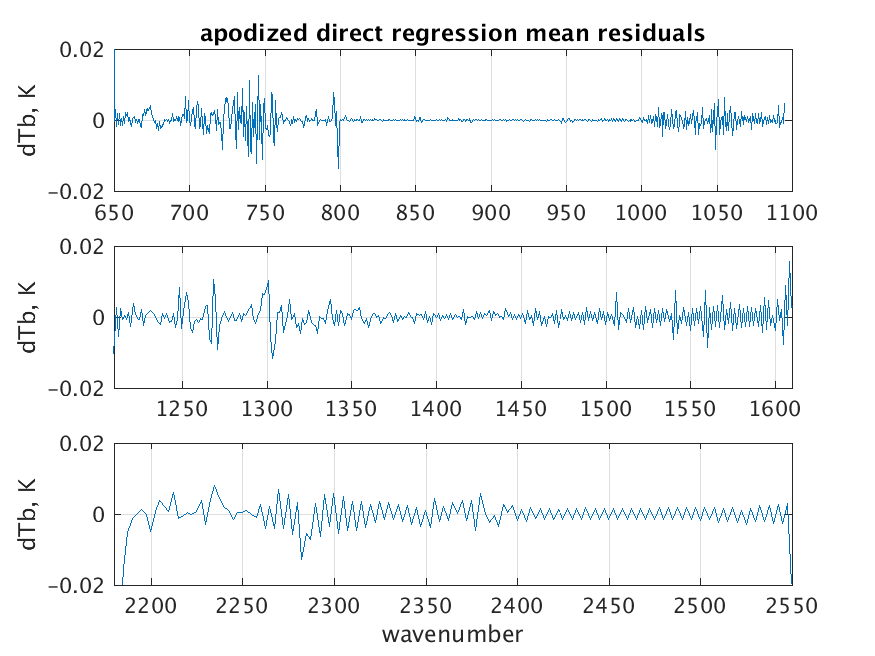
\includegraphics[width=\linewidth]{slackfigs/ap_direct_regr.png}
  \caption{mean residuals for apodized {\airs} to {\cris} direct
    regression}
  \label{dreg1}
\end{figure}

\begin{figure} % source slackfigs a2cris_regr4.m
  \centering
  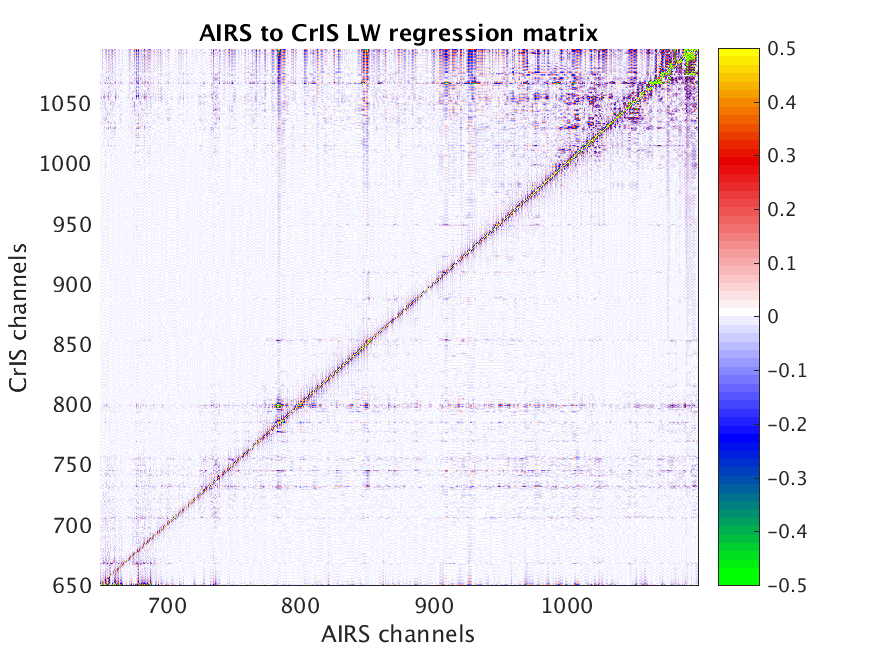
\includegraphics[width=\linewidth]{slackfigs/full_7377_LW_regr_mat.png}
  \caption{regression coefficients for the LW direct regression}
  \label{dreg3}
\end{figure}

% \begin{figure} % source slackfigs a2cris_regr4.m
%   \centering
%   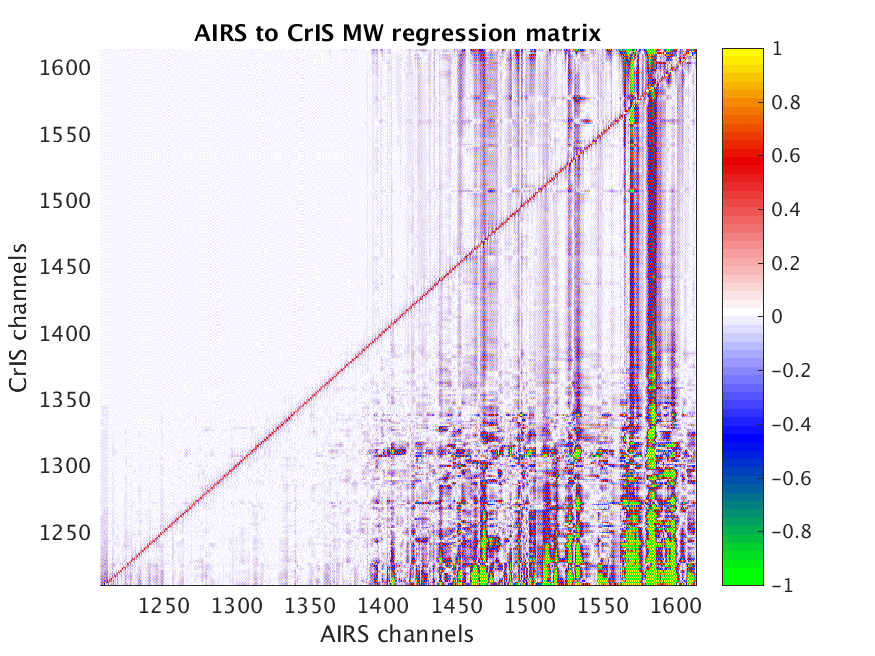
\includegraphics[width=\linewidth]{slackfigs/full_7377_MW_regr_mat.png}
%   \caption{regression coefficients for the MW direct regression}
%   \label{dreg4}
% \end{figure}
% 
% \begin{figure} % source slackfigs a2cris_regr4.m
%   \centering
%   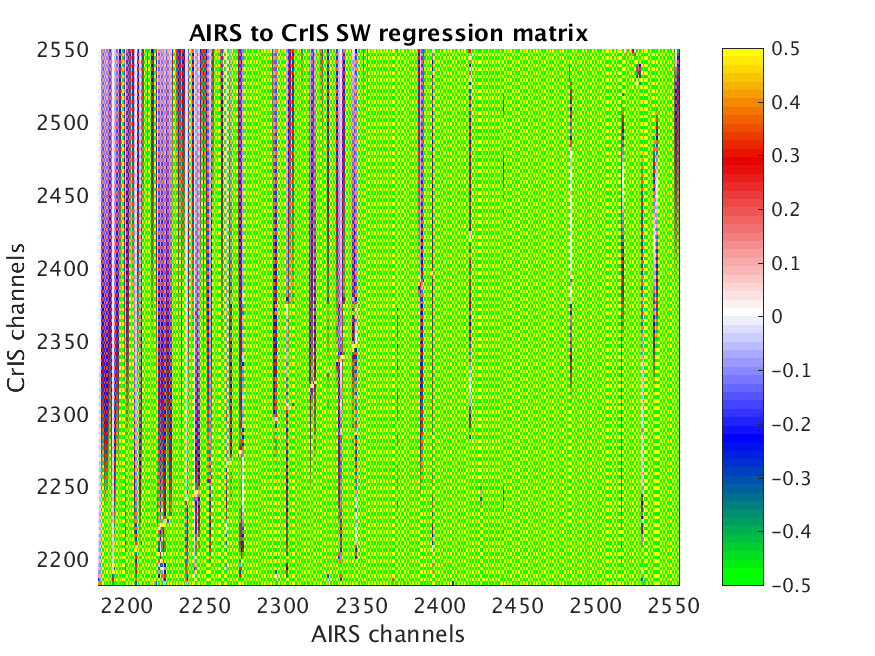
\includegraphics[width=\linewidth]{slackfigs/full_7377_SW_regr_mat.png}
%   \caption{regression coefficients for the SW direct regression}
%   \label{dreg5}
% \end{figure}

\begin{figure} % source slackfigs a2cris_regr5.m
  \centering
  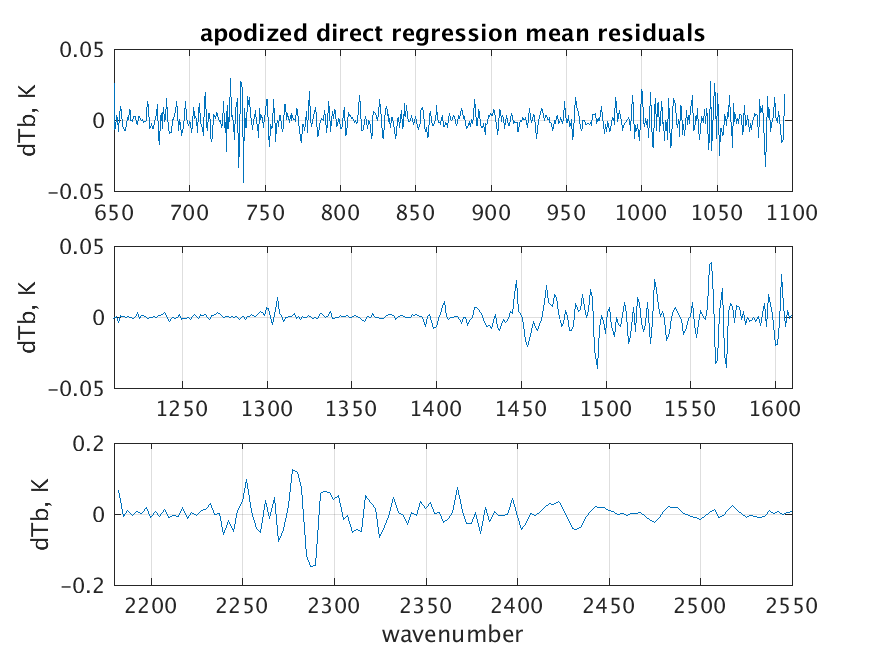
\includegraphics[width=\linewidth]{slackfigs/ap_pc_direct_regr.png}
  \caption{mean residuals for apodized {\airs} to {\cris} principal
    component regression}
  \label{dreg6}
\end{figure}

\begin{figure} % source slackfigs a2cris_regr5.m
  \centering
  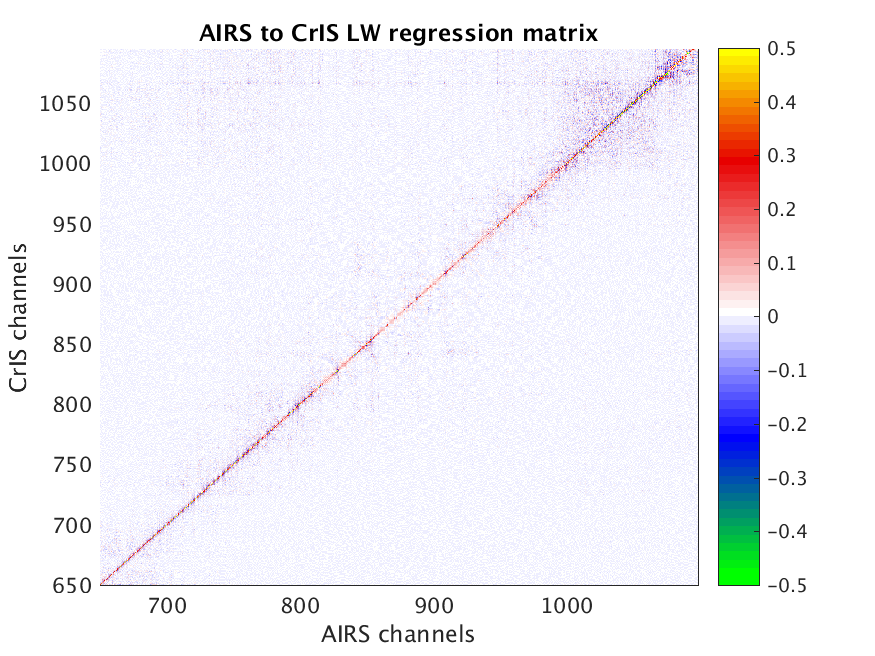
\includegraphics[width=\linewidth]{slackfigs/LW_pc_regr_mat.png}
  \caption{regression coefficients for the LW principal component
    regression}
  \label{dreg7}
\end{figure}

\begin{figure} % source slackfigs a2cris_regr5.m
  \centering
  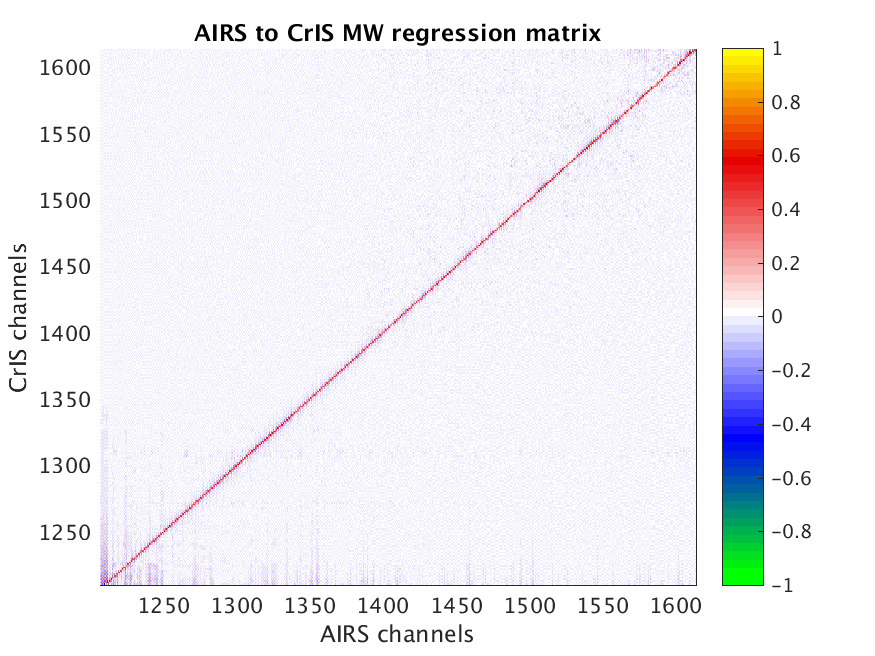
\includegraphics[width=\linewidth]{slackfigs/MW_pc_regr_mat.png}
  \caption{regression coefficients for the MW principal component
    regression}
  \label{dreg8}
\end{figure}

\begin{figure} % source slackfigs a2cris_regr5.m
  \centering
  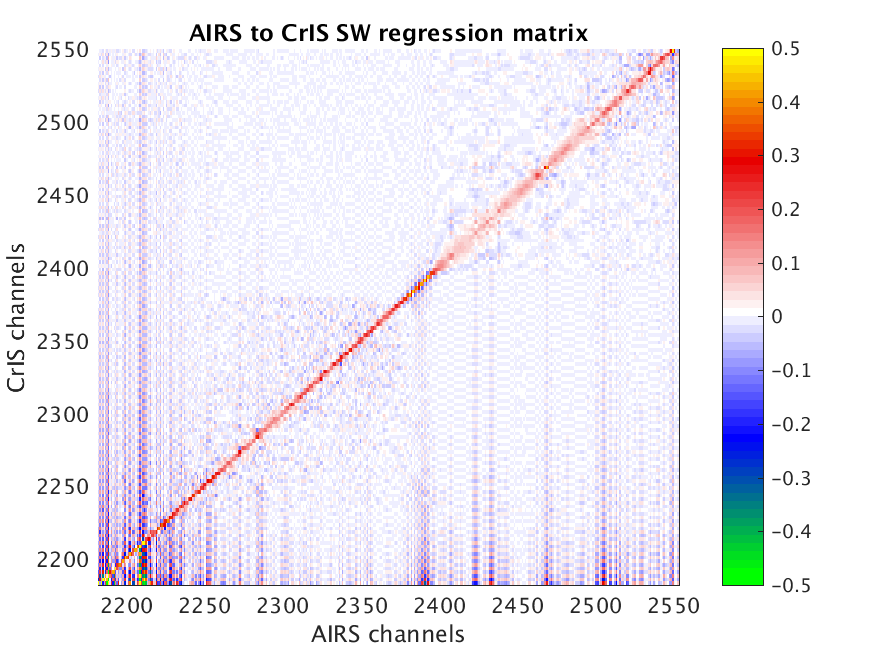
\includegraphics[width=\linewidth]{slackfigs/SW_pc_regr_mat.png}
  \caption{regression coefficients for the SW principal component
    regression}
  \label{dreg9}
\end{figure}

%---------------------------------------------------------------------
\FloatBarrier
\section{Conclusions}
\label{appcon}

We have shown how to take advantage of detailed knowledge of the
{\airs} spectral response functions to deconvolve channel radiances
to a resolution-enhanced intermediate representation, typically a
$0.1$~\wn\ grid.  This deconvolution by itself gives a modest
resolution enhancement at the cost of added artifacts and noise, but
the main application is reconvolution to an alternate instrument
specification.  We consider two cases: reconvolution to the {\cris}
user grid, and to an idealized grating model.  This translation
works well by itself but can be improved with a linear correction
applied independently to each channel, with coefficients determined
by regression.  Finally, we consider principal component regression
directly from {\airs} to {\cris} radiances, and find a tradeoff
between residual size and undesired correlations.  Reducing the
correlations increases the residuals, which become larger than for
translation with deconvolution.

These ideas have been implemented and tested extensively, with
Matlab demo code published on github.  Our demos are i/o bound, but
the in-core time for the {\airs} to {\cris} translation is divided
into roughly 25 percent for the deconvolution and 75 percent for
reconvolution, about 22 seconds to process our 7377 profile cloudy
test set on one compute node.  Calculating the pseudo-inverse adds
another 12 seconds, but that only needs to be done when the
translation parameters change.

\FloatBarrier
\section{Appendix}
\label{append}

We want to measure the correlation of a set of radiances.  One such
measure is dimension of a spanning set.  For an approximation we use
the basis size needed to get reconstruction residuals below some
fixed threshold.  Let $r_0$ be an $m \times n$ array of radiances,
one row per channel and one column per observation.  Let $r_1 = U
S\,V^T$ be a singular value decomposition with singular values in
descending order and $U_k$ the first $k$ columns of $U$.  Let $r_k =
U_k U_k^T r_0$; then $r_k \approx r_0$.  The approximation improves
as $k$ increases and becomes exact for some $k <= m$.  This is the
analog of principal component filtering using left-singular rather
than eigenvectors and is useful as a form of compression when $k$ is
small relative to $n$.  For that case we save $U_k$ and $U_k^T r_0$
separately.  Applications include compression of IASI radiance data
and the kcarta absorption coefficient database.

We use a threshold for equivalence that is relevant for our
applications.  Let $B^{-1}$ be the inverse Planck function and
define $d(r_1, r_2) = \rms(B^{-1}(r_1, v) - B^{-1}(r_2, v))$, the
{\rms} difference over all channels and observations of the
brightness temperatures of radiance data.  Finally let $j$ be the
smallest value such that $d(r_0, r_j) \le T_d$, for some threshold
$T_d$.  Then $j$ is the effective dimension of our set $r_0$.  Here
we have chosen $T_d = 0.02$~K.  For the 49 profile fitting set this
gives $j=48$, which we interpret as largely uncorrelated, while for
the 7377 profile cloudy set we found $j=260$, which we interpret as
highly correlated.

\FloatBarrier
\bibliographystyle{abbrv}
\bibliography{decon_paper}

\end{document}

